\chapter{Planification}

L’idée générale de la planification de la réalisation du projet consiste à pouvoir au plus vite valider le fonctionnement de la chaîne complète de communication. Pour se faire le développement sera découpé en 3 phases.

\begin{itemize}
\item Phase 1 : Validation de la transmission des données avec LoRa
\item Phase 2 : Stockage des données dans la base de données et application mobile simple
\item Phase 3 : Finalisation des fonctionnalités
\end{itemize}

Dans la phase 1, un capteur avec uniquement la fonctionnalité d’acquisition de la position GPS ainsi que de la transmission radio ainsi qu’une passerelle capable de récupérer les données et les afficher simplement sur un terminal seront en priorité développées puis testées. Le test veillera à reproduire les conditions finales d’utilisation du capteur, cela veut dire vérifier que la réception des données est bonne lorsque le capteur est en mouvement.

Au terme de la première phase, un jalon est placé, il implique la validation de la solution choisie en termes de matériel pour le capteur et la passerelle. Si le test de transmission de paquet LoRa avec le capteur en mouvement est concluant alors la solution sera validée. Si au contraire des problèmes sont rencontrés il faudra peut-être changer de matériel.

La phase 2 consiste à développer la base de données, dans son ensemble, ainsi qu’une application mobile simple qui se contentera d’afficher simplement des positions GPS sur une carte. Cela implique également la modification du serveur de paquet qui devra aller écrire les informations dans la base. Une fois implémenté cela permet de faire le test de la chaîne complète et vérifier si la fréquence de transmission des données est suffisante pour garantir une mise à jour en temps réel de la position.

A la fin de la deuxième phase, la solution choisie pour la fréquence de transmission des données sera validée. Elle permettra de définir définitivement la configuration afin d’avoir une réactivité adéquate du système.
Enfin dans la phase 3 toutes les fonctionnalités seront finalisées afin de pouvoir compléter le projet dans son entier. Cela comporte l’ajout de l’acquisition de la fréquence cardiaque ainsi que de la cadence de pas au capteur, la modification du serveur de paquet afin de pouvoir stocker ces nouvelles informations et la finalisation de l’application mobile afin de pouvoir afficher toutes les informations relatives aux coureurs ainsi que les fonctionnalités de gestion d’événements.

Pour terminer, lorsque le développement du système sera achevé, une démonstration de son fonctionnement en extérieur dans des conditions similaire à une course sera fait. Une personne sera équipée du capteur et elle se lancera sur un parcours à définir, d’une longueur entre 5 et 10 km, afin de pouvoir générer des données et les afficher grâce à l’application. Cela permettra de vérifier le bon fonctionnement du système.

Le planning se base sur les heures de travail suivantes.

\begin{itemize}
\item Lundi à Jeudi – 18h00 à 22h00 (4h de travail)
\item Vendredi – 8h00 à 12h00 et 13h00 à 17h00 (8h de travail)
\item Samedi et Dimanche – 14h00 à 18h00 (4h de travail)
\end{itemize}

Suivant l’avancement du travail de Bachelor il me sera possible d’augmenter les heures de travail le Samedi et le Dimanche afin de pouvoir compléter le projet dans le temps imparti. 

%\newpage
%\KOMAoptions{paper=landscape,pagesize}
%\recalctypearea

%\afterpage{
\newpage

\paperwidth=\pdfpageheight
\paperheight=\pdfpagewidth
\pdfpageheight=\paperheight
\pdfpagewidth=\paperwidth
\headwidth=\textheight
\begingroup 
\vsize=\textwidth
\hsize=\textheight
\section{Diagramme de Gantt}

Le diagramme de Gantt~\ref{fig:planning} décrit le planning du projet pour la période de développement et réalisation.

\begin{figure}[h]
\centering
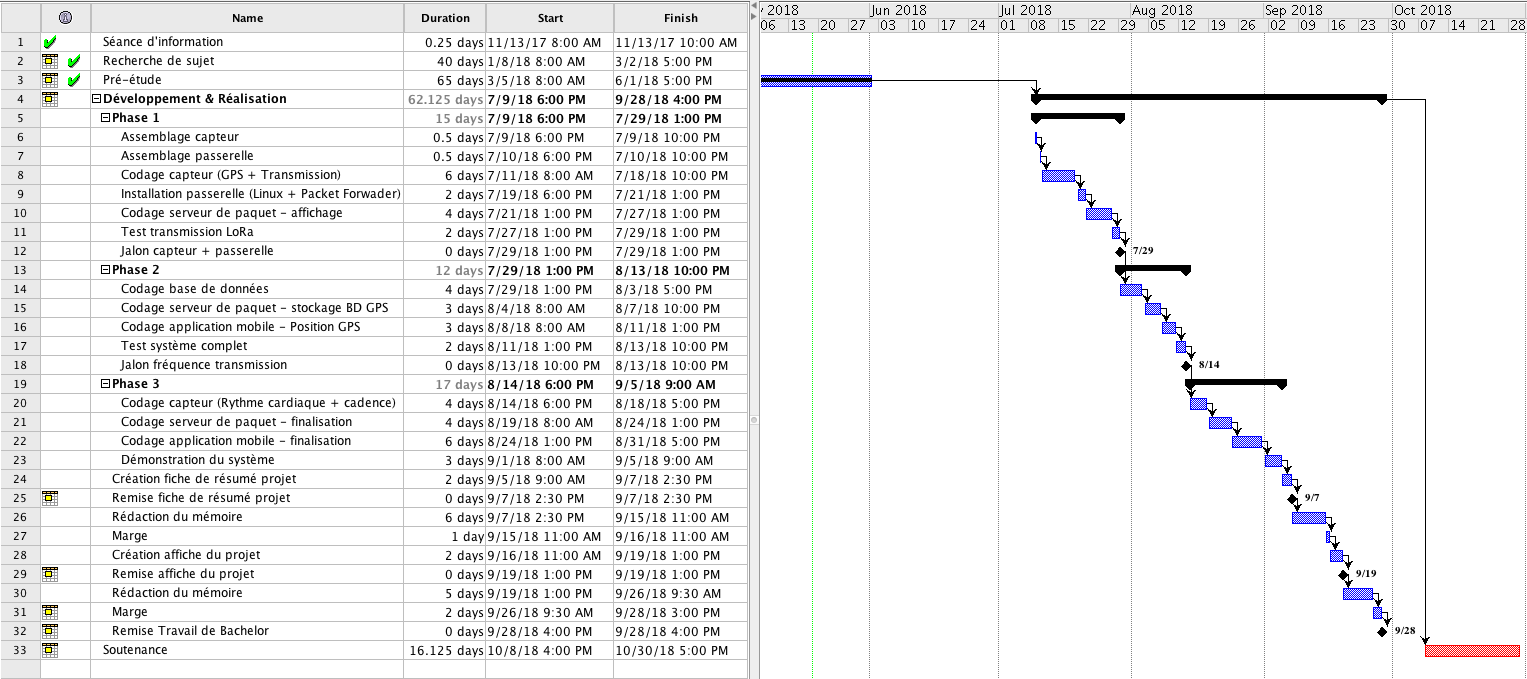
\includegraphics[scale=0.45]{../../planning/gantt_planning.png}
\caption[Planning - Diagramme de Gantt]{Planning - Diagramme de Gantt}
\label{fig:planning}
\end{figure}
\endgroup
\newpage
\paperwidth=\pdfpageheight
\paperheight=\pdfpagewidth
\pdfpageheight=\paperheight
\pdfpagewidth=\paperwidth
\headwidth=\textwidth

%}

%Le diagramme de Gantt~\ref{fig:planning} décrit le planning du projet pour la période de développement et réalisation.
%
%\begin{figure}[htb]
%\centering 
%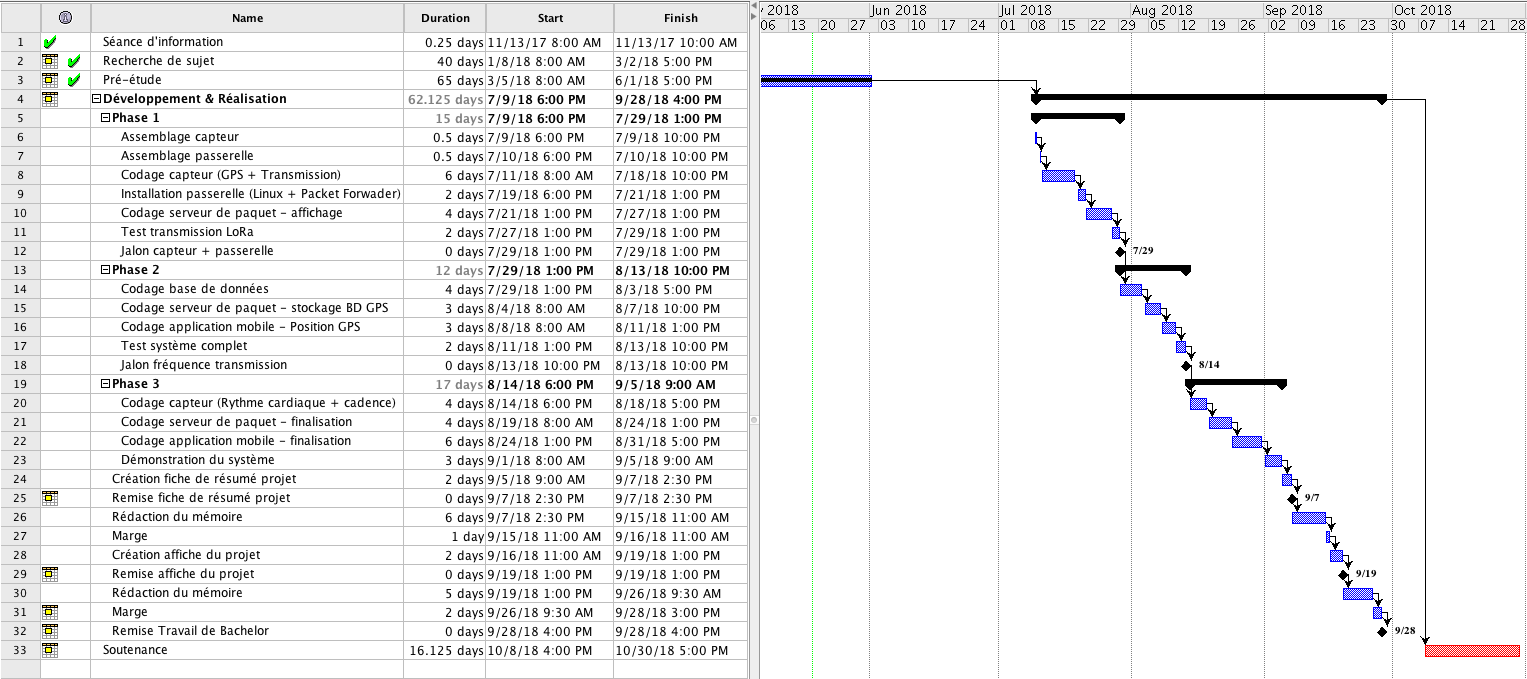
\includegraphics[width=1\columnwidth]{../../planning/gantt_planning.png} 
%\caption[Planning - Diagramme de Gantt]{Planning - Diagramme de Gantt}
%\label{fig:planning}
%\end{figure}

%\newpage
%\KOMAoptions{paper=portrait,pagesize}
%\recalctypearea